% IEEE TALE 2026 — Short Paper (4 pages, A4, double-blind)
% Compile: pdflatex tale2026_short.tex (twice)
\documentclass[conference,a4paper]{IEEEtran}
\usepackage[T1]{fontenc}
\usepackage[utf8]{inputenc}
\usepackage{graphicx}
\usepackage{booktabs}
\usepackage{tikz}
\usetikzlibrary{positioning,arrows.meta}
\usepackage{balance}
\usepackage[hidelinks]{hyperref}

% ===== BENCHMARK RESULT MACROS (filled from bench/results/summary.json) =====
\newcommand{\bAERfull}{100}      % action emission rate, full pipeline (%)
\newcommand{\bAERnoseed}{100}    % action emission rate, no seed (%)
\newcommand{\bAERnoretry}{100}   % action emission rate, no retry (%)
\newcommand{\bAERnosys}{100}     % action emission rate, no system param (%)
\newcommand{\bSPUfull}{37.5}     % spurious action rate, full (%)
\newcommand{\bSPUnoseed}{37.5}
\newcommand{\bSPUnoretry}{37.5}
\newcommand{\bSPUnosys}{37.5}
\newcommand{\bJSONfull}{100}     % JSON validity (%)
\newcommand{\bJSONnoseed}{100}
\newcommand{\bJSONnoretry}{100}
\newcommand{\bJSONnosys}{100}
\newcommand{\bSEMfull}{77.8}     % semantic validity of parsed actions (%)
\newcommand{\bSEMnoseed}{92.0}
\newcommand{\bSEMnoretry}{76.6}
\newcommand{\bSEMnosys}{68.9}
\newcommand{\bINTfull}{10}       % invalid actions intercepted (count)
\newcommand{\bINTnoseed}{4}
\newcommand{\bINTnoretry}{11}
\newcommand{\bINTnosys}{14}
\newcommand{\bRETfull}{0}        % retry rate (%)
\newcommand{\bRETnoseed}{0}
\newcommand{\bRETnosys}{0}
\newcommand{\bTotalCalls}{180}   % total model interactions in benchmark (4B x4 cond + 12B + 70B)
% ============================================================================

\begin{document}

\title{Validate Before You Apply: An LLM-Augmented Learning Assistant with Action Validation for Computer Networks Education}

\author{\IEEEauthorblockN{Anonymous Author(s)}
\IEEEauthorblockA{Submission to IEEE TALE 2026 --- omitted for double-blind review}}

\maketitle

\begin{abstract}
Large language models (LLMs) promise adaptive tutoring, but when a tutoring agent can also act on the learner's working artifact, hallucination acquires a new cost: an incorrect action silently corrupts the very object the student is reasoning about. We present CAPA8, a browser-based learning environment for computer networks education that couples a conversational LLM tutor with an interactive network topology simulator the tutor can read and modify. Its central design contribution is a pedagogical reliability layer: every model-proposed modification is expressed in a closed action grammar, parsed, and validated against the live topology state before it is applied, with ambiguous requests resolved by rule-based clarification dialogues that bypass the LLM entirely. Adaptive scaffolding is provided by a Level\,$\times$\,Focus mode matrix that reconfigures the tutor from step-by-step guidance with analogies to a technical peer. A preliminary technical evaluation combines 47 unit tests covering the validation pipeline with a reliability benchmark of \bTotalCalls{} model interactions across three deployment scenarios---a small and a larger local open-weight model and a cloud-hosted high-capacity model---plus an ablation of the prompt-side mechanisms, showing that the validation layer intercepts all structurally invalid actions across every model while preserving high task completion. A classroom study is planned as future work.
\end{abstract}

\begin{IEEEkeywords}
large language models, intelligent tutoring systems, scaffolding, computer networks education, hallucination mitigation, human--AI collaboration
\end{IEEEkeywords}

\section{Introduction}
Computer networking is taught through abstractions---addressing, subnetting, routing, gateways---whose consequences only become visible when a concrete topology misbehaves. Professional simulators such as Cisco Packet Tracer~\cite{packettracer} and emulation environments such as Mininet~\cite{lantz2010mininet} give students that concreteness, but they carry steep learning curves, and none of them explains \emph{why} the ping the student just issued never arrived. The explanatory gap is usually filled by an instructor, who does not scale, or lately by a general-purpose chatbot, which cannot see the student's diagram and therefore reasons about a network that does not exist.

LLMs have shown clear potential as adaptive explainers in engineering education~\cite{kasneci2023chatgpt,denny2024computing}. The obvious next step---letting the tutor not only explain the student's artifact but also act on it---introduces a reliability problem that is qualitatively different from textual hallucination~\cite{ji2023survey}. A fabricated sentence can be challenged; a fabricated \emph{action} (connecting a PC to a router that does not exist, duplicating an IP address, ``fixing'' a missing gateway by adding a spurious cable) rewrites the learning artifact itself. Novices are the least equipped to detect such corruption: they cannot tell whether the inconsistency they now observe is their own misconception or the tool's error, which undermines both trust and the diagnostic reasoning the exercise was meant to train.

CAPA8 is a no-install, browser-based environment that addresses this problem by treating the LLM as an \emph{untrusted proposer}. The model never mutates the topology directly. It emits proposals in a closed action grammar; a deterministic pipeline classifies the student's intent before any model call, constrains the prompt, parses the response, validates every proposed action against the live graph state, and routes batches through a human-confirmable preview with single-step undo. The same pipeline carries the pedagogy: a Level\,$\times$\,Focus mode matrix adapts the depth and register of explanations, and a topology analyzer injects the same misconfiguration warnings the student sees on the canvas into the model's context, so tutor and student literally look at the same network.

This paper makes three contributions: (1)~the design of a validate-before-apply action pipeline as a pedagogical reliability mechanism for LLM tutors that operate on learner artifacts; (2)~an adaptive scaffolding scheme that operationalizes tutoring styles as a selectable Level\,$\times$\,Focus matrix combined with intent-dependent decoding temperature; and (3)~a preliminary technical evaluation---formal unit verification plus a reliability benchmark spanning three deployment scenarios (small local, larger local, and cloud models) with an ablation of the prompt-side mechanisms---showing that validation intercepts every structurally invalid action regardless of model capability, and quantifying how much each mechanism contributes.

\section{Related Work}
\subsubsection*{LLMs in computing education}
Kasneci et al.~\cite{kasneci2023chatgpt} map the opportunities and risks of LLMs across education, identifying hallucination and overreliance as core concerns. Within computing education, Denny et al.~\cite{denny2024computing} survey the post-GPT landscape, and CodeHelp~\cite{liffiton2023codehelp} demonstrates guardrails that keep an LLM helper from emitting full solutions in programming classes. CodeHelp's guardrails shape the \emph{text} a model returns; CAPA8 extends the guardrail idea to \emph{state-changing actions}, where the failure mode is not an unwanted answer but a corrupted artifact.

\subsubsection*{Scaffolding and intelligent tutoring systems}
The tutor configurations in CAPA8 instantiate classic scaffolding theory: graduated assistance within the learner's zone of proximal development~\cite{vygotsky1978mind,wood1976role}, software realizations of structuring and problematizing supports~\cite{reiser2004scaffolding}, and the ITS tradition of step-based adaptive dialogue~\cite{vanlehn2011relative}. CAPA8 differs from end-to-end LLM tutors in deliberately keeping parts of the dialogue deterministic: ambiguity resolution and misconfiguration detection are rule-based, reserving the LLM for explanation and proposal generation.

\subsubsection*{Constraining LLM output}
Hallucination surveys~\cite{ji2023survey} motivate a growing toolbox of output constraints, from programmable conversational rails~\cite{rebedea2023nemo} to constrained semantic decoding for code~\cite{poesia2022synchromesh}. These techniques operate at generation time and are stateless with respect to the application. CAPA8 adds a complementary, state-dependent stage: semantic validation of each proposed action against the live topology (referential integrity, duplicate addresses, type normalization), plus a human confirmation step consistent with human--AI interaction guidelines~\cite{amershi2019guidelines}. To our knowledge this validate-before-apply pattern has not been reported for network-education tools, whose mainstream representatives~\cite{packettracer,lantz2010mininet,kurose2021computer} offer no integrated conversational tutoring at all.

\section{System Design}
\subsection{Architecture Overview}
CAPA8 is a dependency-light web application (vanilla ES6 modules, no build step) with two surfaces that share one conversation store: a chat page for open tutoring and a topology simulator with an embedded tutor panel. The simulator supports ten device types (router, switch, PC, firewall, server, cloud, access point, and three industrial nodes: PLC, robot arm, AGV), link properties (latency, bandwidth, loss), a virtual terminal (\texttt{ping}, \texttt{traceroute}, \texttt{ipconfig}, ARP and routing inspection) animated over the graph, and eleven curated example topologies (LAN, VLAN routing, DMZ, campus, data center, industrial). A Node.js backend relays prompts to either a cloud provider or a locally hosted open-weight model, so institutions can run the entire stack on commodity hardware without sending student data to third parties.

Two design decisions tie the architecture to pedagogy. First, a static topology analyzer continuously detects eight classes of misconfiguration (duplicate IPs, isolated nodes, missing gateways, downed or lossy links, disconnected components) and renders them to the student; the identical issue list is serialized into the LLM context, so the tutor's explanations refer to the same evidence the student can see. Second, conversation state persists across both surfaces, allowing a student to design a network in the chat, open it in the simulator, and continue the same dialogue.

\begin{figure}[t]
\centering
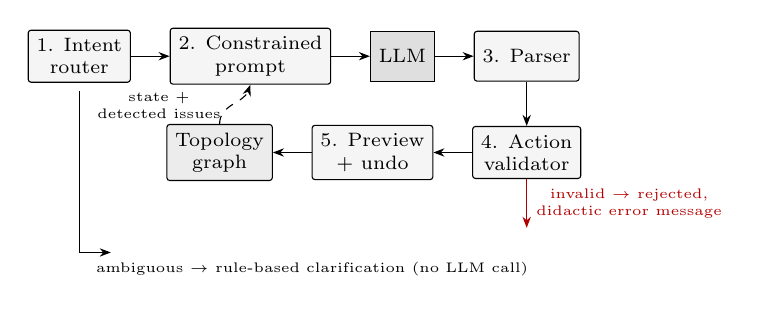
\begin{tikzpicture}[
  font=\scriptsize,
  stage/.style={draw, rounded corners=1pt, align=center, inner sep=3pt, minimum height=18pt, fill=gray!8},
  llm/.style={draw, align=center, inner sep=3pt, minimum height=18pt, fill=gray!25},
  arr/.style={-{Stealth[length=4pt]}},
  lbl/.style={font=\tiny, align=center},
  node distance=10pt and 14pt]
\node[stage] (intent) {1. Intent\\router};
\node[stage, right=of intent] (prompt) {2. Constrained\\prompt};
\node[llm, right=of prompt] (llm) {LLM};
\node[stage, right=of llm] (parse) {3. Parser};
\node[stage, below=16pt of parse] (valid) {4. Action\\validator};
\node[stage, left=of valid] (preview) {5. Preview\\+ undo};
\node[stage, left=of preview, fill=gray!15] (graph) {Topology\\graph};
\draw[arr] (intent) -- (prompt);
\draw[arr] (prompt) -- (llm);
\draw[arr] (llm) -- (parse);
\draw[arr] (parse) -- (valid);
\draw[arr] (valid) -- (preview);
\draw[arr] (preview) -- (graph);
\draw[arr, dashed] (graph.north) to[out=90,in=-110] node[lbl, left, pos=0.45]{state +\\detected issues} (prompt.south);
\draw[arr] ([yshift=-3pt]intent.south) |- node[lbl, below right=0pt and -2pt, pos=0.7]{ambiguous $\to$ rule-based clarification (no LLM call)} ++(0.4,-2.05);
\draw[arr, red!70!black] (valid.south) -- node[lbl, right, text=red!70!black]{invalid $\to$ rejected,\\didactic error message} ++(0,-0.62);
\end{tikzpicture}
\caption{The validate-before-apply pipeline. The LLM only proposes; deterministic stages decide what reaches the learner's topology.}
\label{fig:pipeline}
\end{figure}

\subsection{Adaptive Scaffolding: the Level\texorpdfstring{\,$\times$\,}{x}Focus Matrix}
Tutoring style is the product of a three-step \emph{Level} and a two-value \emph{Focus} (Table~\ref{tab:modes}), yielding six configurations that are compiled into the system prompt. Levels encode scaffolding intensity in the sense of graduated, fadeable support~\cite{wood1976role,reiser2004scaffolding}: the guided level forbids unexplained acronyms, requires analogies, warns about typical novice errors, and ends each turn with a reflection question; the technical level addresses the student as a peer and cites RFC/IEEE standards. Focus selects the task frame: \emph{design} (constructive: propose and build topologies) or \emph{troubleshoot} (diagnostic: locate and explain faults). Decoding temperature is additionally bound to intent---0.0 for modifications, 0.2 for conceptual explanation---so creative variability is spent on pedagogy, never on state changes.

\begin{table}[t]
\caption{Scaffolding configurations (Level $\times$ Focus)}
\label{tab:modes}
\centering
\scriptsize
\begin{tabular}{@{}lp{5.6cm}@{}}
\toprule
\textbf{Level} & \textbf{Tutor behavior (applies to both foci)} \\
\midrule
Guided & Step-by-step, simple analogies, no unexplained acronyms, anticipates novice errors, closes with a reflection question. \\
Balanced & Direct and practical; at most three paragraphs or a concise list. \\
Technical & Dense, standards-referenced (RFC/IEEE), proactively flags design faults, peer register. \\
\midrule
\textbf{Focus} & \emph{Design}: propose and construct topologies. \emph{Troubleshoot}: analyze the graph, explain faults, propose concrete fixes. \\
\bottomrule
\end{tabular}
\end{table}

\subsection{Deterministic Intent Routing and Clarification}
Before any model call, a rule-based classifier assigns each utterance one of six intents: \emph{conceptual}, \emph{graph query}, \emph{diagnostic}, \emph{clear modification}, \emph{ambiguous modification}, or \emph{full-graph application}. Classification uses imperative-verb lexicons, question patterns, and---characteristically---the live graph: a message is a \emph{clear} modification only if it references existing node labels or a concrete target. Ambiguous requests (``add a device somewhere'') never reach the LLM; instead, a clarification dialogue is generated from the graph itself, offering the available attachment points as options. This keeps a class of interactions instant, free, and perfectly predictable, in the tradition of step-based ITS dialogue moves~\cite{vanlehn2011relative}, and it determines downstream policy: which prompt blocks are injected, which temperature is used, and whether the action grammar is enabled at all.

\subsection{Action Grammar and the Validation Layer}
All state changes are expressed in a closed grammar of seven actions (\texttt{add\_node}, \texttt{add\_link}, \texttt{update\_node}, \texttt{delete\_node}, \texttt{delete\_link}, \texttt{set\_link\_status}, \texttt{apply\_graph}) serialized as JSON inside explicit \texttt{[CAPA8\_ACTION]} delimiters. Three prompt-side mechanisms raise the probability that an action request actually yields well-formed blocks: a directive with paired wrong/correct counter-examples (e.g., gateway repair must patch a node property, never add a cable), a seeded exchange of canonical examples injected only for action intents, and an automatic single retry with a stricter instruction when an expected action is missing.

What the model returns is still untrusted. A parser isolates the delimited blocks (malformed JSON is marked invalid and can never execute) and strips them from the text shown to the student. Each surviving action then passes semantic validation against the current graph: the action type must belong to the whitelist; referenced source and target nodes must exist; duplicate IP assignments and duplicate links are flagged; unknown device types are normalized through an alias table (\texttt{laptop}\,$\to$\,\texttt{pc}, \texttt{internet}\,$\to$\,\texttt{cloud}); and an \texttt{add\_node} naming an existing node is rewritten into an \texttt{update\_node}, converting the most frequent duplication hallucination into the action the model should have chosen. Rejected actions are not silently dropped: the validator emits an explanatory message in the chat (``source node \emph{Router5} not found''), turning the failure into feedback for both the student and, via history, the model. During batch application, validation re-runs per action against the refreshed graph, so earlier actions in a batch cannot smuggle later ones past the checks.

\subsection{Human-in-the-Loop Application}
Validated actions still require consent at the right granularity. Batches of three or more actions open a preview panel where the student reviews and confirms the plan; any applied batch is one atomic undo step; and the frontend ignores all model-proposed canvas coordinates, retaining layout authority on the client. These choices follow established human--AI interaction guidance on efficient correction and graceful degradation~\cite{amershi2019guidelines}: the system makes the tutor's agency visible, bounded, and reversible---properties we consider preconditions for trusting an acting tutor in a classroom.

\section{Preliminary Evaluation}
\subsection{Formal Verification of the Pipeline}
The deterministic pipeline components are covered by 47 unit tests (validator, intent router, response parser, graph model), all passing. The validator tests certify the properties the reliability argument rests on: nonexistent references are rejected, unknown action and device types are rejected, alias normalization and the \texttt{add\_node}-to-\texttt{update\_node} rewrite behave as specified, and duplicate IPs raise warnings.

\subsection{Reliability Benchmark}
We probed the end-to-end pipeline with a scripted benchmark of 30 student-style utterances in Spanish against a fixed five-node topology seeded with deliberate faults (a PC without gateway, a PC without IP, an in-use IP address). The suite contains 16 clear modification requests (including traps: repairing the missing gateway, assigning the missing IP, referencing nonexistent devices, reusing an occupied IP), 6 diagnostic requests, and 8 conceptual or query utterances for which any emitted action is spurious. Every response was parsed and validated by the production code itself; in total \bTotalCalls{} model interactions were evaluated.

\subsubsection*{Across deployment scenarios}
We ran the full pipeline under three scenarios spanning the privacy/cost spectrum a school faces: a small local model (Gemma~3~4B~\cite{gemmateam2025gemma3}), a larger local model (Gemma~3~12B), both served through Ollama on commodity hardware, and a cloud-hosted high-capacity model (Llama~3.3~70B via Groq). Table~\ref{tab:models} reports the results. All three emit an action for every modification request and every emitted block is well-formed JSON, yet none is free of \emph{semantically} invalid actions: 10 to 12 actions per model referenced a nonexistent node or duplicated an address and were intercepted before reaching the graph. Model capability changes \emph{which} failure mode dominates---the 4B model wrongly emits actions on 37.5\% of conceptual prompts, whereas neither larger model ever does---but it does not remove the need for validation: even the 70B cloud model produced eleven structurally invalid actions, all caught. Interception is by construction independent of model quality.

\begin{table}[t]
\caption{Full pipeline across deployment scenarios (30 prompts each)}
\label{tab:models}
\centering
\scriptsize
\begin{tabular}{@{}llccccc@{}}
\toprule
\textbf{Model} & \textbf{Deploy.} & \textbf{AER\,\%} & \textbf{Spur.\,\%} & \textbf{JSON\,\%} & \textbf{Valid\,\%} & \textbf{Interc.} \\
\midrule
Gemma 3 4B    & Local & 100 & 37.5 & 100 & 77.8 & 10 \\
Gemma 3 12B   & Local & 100 & 0.0  & 100 & 66.7 & 12 \\
Llama 3.3 70B & Cloud & 100 & 0.0  & 100 & 80.0 & 11 \\
\bottomrule
\multicolumn{7}{@{}p{8.2cm}@{}}{\tiny Columns as in Table~\ref{tab:bench}. Local models served via Ollama on commodity hardware; the cloud model via Groq. Every model emits well-formed actions for all requests, yet none avoids semantically invalid ones, all intercepted before reaching the graph.}
\end{tabular}
\end{table}

\subsubsection*{Ablation of the prompt-side mechanisms}
To isolate each prompt-side mechanism we ablated them on the smallest and hardest case, Gemma~3~4B, where structured-output reliability is most fragile: the full pipeline, no seeded examples, no auto-retry, and the directive moved from the system channel into the user prompt (Table~\ref{tab:bench}). Routing the directive through the system channel is the dominant aid---removing it raises intercepted actions from 10 to 14 and drops semantic validity to 68.9\%. The seeded examples and auto-retry show no clear benefit at this model size (the model already emits an action for every request, so the retry never fires), a candid result we report rather than overstate. The validator's interception nevertheless holds across all four conditions.

\begin{table}[t]
\caption{Ablation of prompt-side mechanisms, Gemma 3 4B local (30 prompts per condition)}
\label{tab:bench}
\centering
\scriptsize
\begin{tabular}{@{}lccccc@{}}
\toprule
\textbf{Condition} & \textbf{AER\,\%} & \textbf{Spur.\,\%} & \textbf{JSON\,\%} & \textbf{Valid\,\%} & \textbf{Interc.} \\
\midrule
Full pipeline & \bAERfull & \bSPUfull & \bJSONfull & \bSEMfull & \bINTfull \\
-- seeded examples & \bAERnoseed & \bSPUnoseed & \bJSONnoseed & \bSEMnoseed & \bINTnoseed \\
-- auto-retry & \bAERnoretry & \bSPUnoretry & \bJSONnoretry & \bSEMnoretry & \bINTnoretry \\
-- system channel & \bAERnosys & \bSPUnosys & \bJSONnosys & \bSEMnosys & \bINTnosys \\
\bottomrule
\multicolumn{6}{@{}p{8.2cm}@{}}{\tiny AER: share of the 16 modification prompts answered with at least one parseable action. Spur.: share of the 8 conceptual/query prompts that wrongly emitted actions. JSON: well-formed blocks among all emitted blocks. Valid: parsed actions passing semantic validation. Interc.: invalid actions intercepted by the validator (would otherwise have corrupted the graph).}
\end{tabular}
\end{table}

The trap items show the division of labor between prompt-side steering and validation: the duplicate-IP and nonexistent-device traps were caught by the validator (as a warning and as didactic rejections, respectively), whereas the gateway and IP-repair traps were answered with the correct property-patch action rather than the spurious-cable shortcut---an outcome attributable to the counter-example prompt blocks, not to validation.

\subsection{Illustrative Scenario}
A student loads the faulty LAN and asks, in troubleshoot focus and guided level, why PC1 cannot reach another subnet. The analyzer has already flagged the empty gateway and that flag travels inside the model context; the tutor explains gateways with an analogy and proposes a one-action fix patching \texttt{PC1.gateway}. Had it proposed a cable to a nonexistent ``Router5'' instead, the validator would have rejected it with an explanatory message, and nothing would have touched the student's network. The student applies the fix (one undo step), reruns \texttt{ping} in the virtual terminal, and watches the packet animation succeed.

\section{Discussion and Limitations}
The validation layer guarantees \emph{structural} soundness, not pedagogical optimality. The gateway trap delineates the boundary precisely: connecting PC1 to the router with a new cable is structurally valid yet didactically wrong; CAPA8 currently steers the model away from it with counter-examples and analyzer hints, but the validator alone would not catch it. Encoding such domain-pedagogical rules (e.g., ``gateway problems are property problems'') as first-class validations is a natural next step. The benchmark, while reproducible and run through the production code path, covers three models, one topology, and Spanish utterances only; it measures reliability, not learning. No claims about learning outcomes are made: the evaluation of comprehension gains, trust calibration, and scaffolding-level effects requires the classroom study outlined below. Finally, we believe the validate-before-apply pattern transfers directly to other artifact-centric subjects---electronic circuits, database schemas, chemical process diagrams---wherever an LLM tutor is allowed to touch the thing the student is building.

\section{Conclusion and Future Work}
CAPA8 demonstrates that an LLM tutor can be given hands---the ability to construct and repair the learner's network topology---without inheriting the model's unreliability, by interposing deterministic intent routing, a closed action grammar, state-aware semantic validation, and human-confirmable application between proposal and effect. Preliminary technical evidence (47 passing unit tests; a \bTotalCalls-interaction benchmark spanning local 4B and 12B models and a 70B cloud model) indicates that the validation layer intercepts every structurally invalid action regardless of model capability, that larger models reduce spurious emissions but never eliminate the invalid actions the validator must catch, and that the architecture runs on hardware schools already own. The next step is a controlled classroom study with networking students (pre/post concept inventory, usability, and scaffolding-level comparison), to be conducted under institutional ethics review. This paper reports no human-subjects data.

\section*{Acknowledgment}
\textit{AI use disclosure (per IEEE and TALE policy):} portions of this manuscript were drafted and edited with the assistance of a generative AI system (Claude, Anthropic), used for text composition, benchmark scripting, and LaTeX formatting under the direction of the authors, who reviewed, verified, and take full responsibility for all content, code, and results. The CAPA8 system itself was designed and implemented by the authors. [Names, affiliations, funding, and the public code repository are withheld for double-blind review and will be restored upon acceptance.]

\balance
\begin{thebibliography}{15}
\bibitem{kasneci2023chatgpt} E. Kasneci \emph{et al.}, ``ChatGPT for good? On opportunities and challenges of large language models for education,'' \emph{Learning and Individual Differences}, vol. 103, p. 102274, 2023.
\bibitem{denny2024computing} P. Denny \emph{et al.}, ``Computing education in the era of generative AI,'' \emph{Communications of the ACM}, vol. 67, no. 2, pp. 56--67, 2024.
\bibitem{liffiton2023codehelp} M. Liffiton, B. Sheese, J. Savelka, and P. Denny, ``CodeHelp: Using large language models with guardrails for scalable support in programming classes,'' in \emph{Proc. 23rd Koli Calling Int. Conf. on Computing Education Research}, 2023, pp. 1--11.
\bibitem{ji2023survey} Z. Ji \emph{et al.}, ``Survey of hallucination in natural language generation,'' \emph{ACM Computing Surveys}, vol. 55, no. 12, pp. 1--38, 2023.
\bibitem{vygotsky1978mind} L. S. Vygotsky, \emph{Mind in Society: The Development of Higher Psychological Processes}. Cambridge, MA: Harvard University Press, 1978.
\bibitem{wood1976role} D. Wood, J. S. Bruner, and G. Ross, ``The role of tutoring in problem solving,'' \emph{Journal of Child Psychology and Psychiatry}, vol. 17, no. 2, pp. 89--100, 1976.
\bibitem{reiser2004scaffolding} B. J. Reiser, ``Scaffolding complex learning: The mechanisms of structuring and problematizing student work,'' \emph{Journal of the Learning Sciences}, vol. 13, no. 3, pp. 273--304, 2004.
\bibitem{vanlehn2011relative} K. VanLehn, ``The relative effectiveness of human tutoring, intelligent tutoring systems, and other tutoring systems,'' \emph{Educational Psychologist}, vol. 46, no. 4, pp. 197--221, 2011.
\bibitem{rebedea2023nemo} T. Rebedea, R. Dinu, M. Sreedhar, C. Parisien, and J. Cohen, ``NeMo Guardrails: A toolkit for controllable and safe LLM applications with programmable rails,'' in \emph{Proc. EMNLP 2023: System Demonstrations}, 2023, pp. 431--445.
\bibitem{poesia2022synchromesh} G. Poesia \emph{et al.}, ``Synchromesh: Reliable code generation from pre-trained language models,'' in \emph{Proc. Int. Conf. on Learning Representations (ICLR)}, 2022.
\bibitem{amershi2019guidelines} S. Amershi \emph{et al.}, ``Guidelines for human--AI interaction,'' in \emph{Proc. CHI Conf. on Human Factors in Computing Systems}, 2019, pp. 1--13.
\bibitem{packettracer} Cisco Networking Academy, ``Cisco Packet Tracer,'' 2024. [Online]. Available: \url{https://www.netacad.com/courses/packet-tracer}
\bibitem{lantz2010mininet} B. Lantz, B. Heller, and N. McKeown, ``A network in a laptop: Rapid prototyping for software-defined networks,'' in \emph{Proc. 9th ACM SIGCOMM Workshop on Hot Topics in Networks (HotNets-IX)}, 2010, pp. 1--6.
\bibitem{kurose2021computer} J. F. Kurose and K. W. Ross, \emph{Computer Networking: A Top-Down Approach}, 8th ed. Hoboken, NJ: Pearson, 2021.
\bibitem{gemmateam2025gemma3} Gemma Team, Google DeepMind, ``Gemma 3 technical report,'' \emph{arXiv preprint arXiv:2503.19786}, 2025.
\end{thebibliography}

\end{document}
